\documentclass{article}

% Language setting
% Replace `english' with e.g. `spanish' to change the document language
\usepackage[utf8]{inputenc}
\usepackage[russian]{babel}

% Set page size and margins
% Replace `letterpaper' with `a4paper' for UK/EU standard size
\usepackage[a4paper,top=2cm,bottom=2cm,left=3cm,right=3cm,marginparwidth=1.75cm]{geometry}

% Useful packages
\usepackage{amsmath}
\usepackage{graphicx}
\usepackage[colorlinks=true, allcolors=blue]{hyperref}
\usepackage{listings}
\usepackage{float   }

\lstdefinestyle{C}{               
    numbers=left,
    numbersep=10pt,
    breaklines=true
}

\title{Дерево ван Эмде Боаса}
\author{Голобородько Димитрий}

\begin{document}
\maketitle


\section{Введение}
\subsection{Суть и назначение}
Дерево ван Эмде Боаса — поисковая структура данных, представляющая собой дерево поиска, позволяющее хранить уникальные целые неотрицательные числа в интервале $[0;2^k)$ и осуществлять над ними основные операции поисковой структуры данных за $O(log{k})$ при затратах памяти $\Theta(2^k)$.
\subsection{История}
Структура разработана осенью 1974 года Питером ван Эмде Боасом во время его трёхмесячного пост-докторского резиденства в Корнеллском университете и представлена в 1975 году. Автор структуры отмечает, что на его ранние публикации оказывал влияние культурный климат в алгоритмике середины 1970-х годов, на фоне которого структура была разработана для машины указателей (pointer machine). Причина в том, что рекурсивный подход требует адресных вычислений. Данные операции не допускались в модели машины с произвольным доступом (RAM), которая была стандартной моделью в развивающейся области исследований проектирования и анализа алгоритмов в 1974 году. Недостатком этого подхода является то, что он приводит к довольно сложным алгоритмам, которые и сегодня трудно корректно реализовать. 
\subsection{Применение}
Данное дерево может применяться в задачах, где требуется поисковая структура данных для множества уникальных целых неотрицаетльных чисел, верхняя граница которого известна заранее, либо ограничена типом данных, при этом количество чисел достаточно велико, чтобы оправдать накладные расходы памяти.
В сети встречаются упоминания применения дерева ван Эмде Боаса в алгоритмах на графах и вычислительной геометрии, а также в сетевых маршрутизаторах.
\section{Описание}
\subsection{Поддерживаемые операции}
\begin{itemize}
    \item member - проверка наличия числа в структуре
    \item insert - вставка числа
    \item remove - удаление числа
    \item successor - поиск следующего по возрастанию числа за данным
    \item predecessor - поиск следующего по убыванию числа за данным
    \item min, max - посик минимального, максимального хранимых чисел 
\end{itemize}
\subsection{Вспомогательные функции}
Для поддержки тех размерностей поддеревьев, из значений которых целый квадратный корень не извлекается, введены следующие вспомогательные функции:
\begin{itemize}
    \item lower\_sqrt(x) - ''нижний квадратный корень'', равен $2^{\lfloor\log_{2}(x)/2\rfloor}$
    \item upper\_sqrt(x) - ''верхний квадратный корень'', равен $2^{\lceil\log_{2}(x)/2\rceil}$
\end{itemize}
При этом $x = upper\_sqrt(x) * lower\_sqrt(x)$, а когда $\sqrt{x}$ - целое, верно $\sqrt{x} = upper\_sqrt(x) = lower\_sqrt(x)$
\begin{itemize}
    \item low(u, x) - младшие $2^{\lfloor\log_{2}(u)/2\rfloor}$ бит номера элемента x, вычисляются как $\lfloor{x/lower\_sqrt(u)}\rfloor$ где u - размерность текущего поддерева
    \item high(u, x) - старшие $2^{\lceil\log_{2}(u)/2\rceil}$ бит номера x, вычисляются как $x\mod{lower\_sqrt()}$  где u - размерность текущего поддерева
    \item index(u, x, y) - совмещает номер элемента из старших бит x и младших бит y, вычисляется как $x*lower\_sqrt(u) + y$, где u - размерность текущего поддерева
    
\end{itemize}
\subsection{Структура данных}
Дерево ван Эмде Боаса является рекурсивной структурой, каждый узел которого является корнем поддерева и содержит в себе:
\begin{itemize}
    \item u - размерность поддерева, элементов
    \item min, max - хранят минимальный и максимальный элемент поддерева
    \item summary - указатель на справочную структуру, которая также является деревом ван Эмде Боаса с размерностью $upper\_sqrt(u)$ элементов 
    \item cluster - массив из $upper\_sqrt(u)$ указателей на поддеревья с размерностью $upper\_sqrt(u)$
\end{itemize}

\begin{figure}[H]
    \centering
    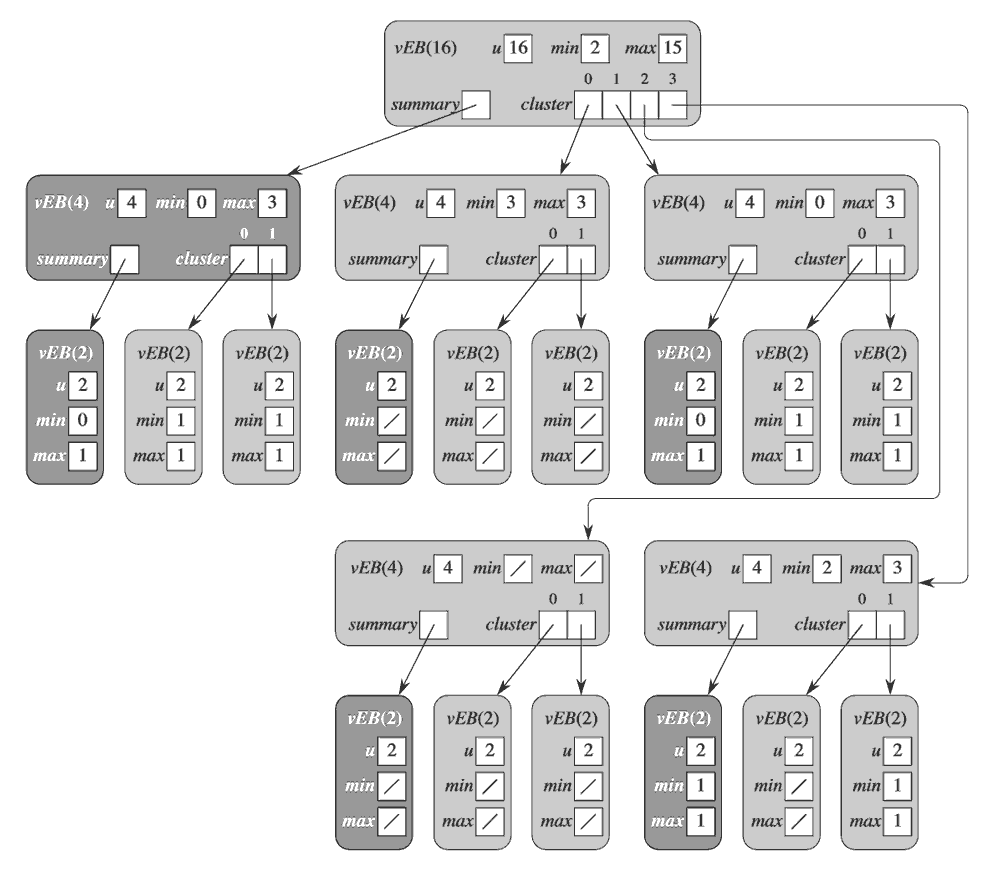
\includegraphics[width=0.9\textwidth]{veb.png}
    \caption{Дерево ван Эмде Боаса размерностью 16, содержащее числа \{2, 3, 4, 5, 7, 14, 15\}}
\end{figure}

\subsection{Входные данные и ограничения}
Оргинальная структура, представленная Питером ван Эмде Боасом требует корректности входных данных, а именно, не гарантирует корректного удаления не существующего элемента, добавления уже существующего элемента. Размерность дерева u должна быть степенью числа 2. Все операции на дереве размерностью u подразумевают работу только с числами из интервала $[0;u)$.
\section{Формальная постановка задачи}
Исследовать и реализовать дерево ван Эмде Боаса в виде набора функций для создания и удаления рекурсивной структуры дерева, исполнения набора поддерживаемых операций (member, insert, remove, successor, predecessor, min, max).
\section{Реализация}
В реализации в рамках данного доклада для значения элемента выбран тип unsigned int, что ограничивает максимальную размерность дерева значением в $2^{32}-1$ элементов, при этом последний элемент unsigned int ($2^{32}-1$) зарезервирован как флаг, обозначающий пустой элемент NIL в полях min и max.
\subsection{Структура узла}
\begin{lstlisting}[language=C,style=C]
typedef struct veb_node veb;
struct veb_node
{
    unsigned int u;
    unsigned int min;
    unsigned int max;
    veb *summary;
    veb **cluster;
};
\end{lstlisting}
\subsection{Реализация вспомогательных функций}
\begin{lstlisting}[language=C,style=C]
const unsigned int NIL = -1;

unsigned int veb_upper_sqrt(unsigned int u) {
    return pow(2, ceil(log2(u)/2));
}

unsigned int veb_lower_sqrt(unsigned int u) {
    return pow(2, floor(log2(u)/2));
}

unsigned int veb_high(unsigned int u,  unsigned int x) {
    return floor(x/veb_lower_sqrt(u));
}

unsigned int veb_low(unsigned int u, unsigned int x) {
    return x % veb_lower_sqrt(u);
}

unsigned int veb_index(unsigned int u, unsigned int x, unsigned int y) {
    return x*veb_lower_sqrt(u)+y;
}
\end{lstlisting}
\subsection{Min, max}
Значения минимума и максимума дерева ван Эмде Боаса, хрянятся в полях структуры корня, поэтому могут быть получены за константное время.
\begin{lstlisting}[language=C,style=C]
unsigned int veb_tree_minimum(veb* v) {
    return v->min;
}
unsigned int veb_tree_maximum(veb* v) {
    return v->max;
}
\end{lstlisting}
\subsection{Member}
\begin{lstlisting}[language=C,style=C]
unsigned int veb_tree_member(veb* v, unsigned int x){
    return
        x == v->min || x == v->max ? 1 :
        v->u == 2 ? 0 :
        veb_tree_member(v->cluster[veb_high(v->u,x)], veb_low(v->u, x));
}
\end{lstlisting}
Строка 3 проверяет случай, в котором искомый элемент x является максимальным или минимальным в дереве, и возвращает истину, если это так. Строка 4 проверяет случай, в котором поддерево размерностью $u=2$ не имеет элементов, возвращает ложь если это так. В противном случае происходит рекурсивное углубление в поддерево с индексом high(u, x) и поиск числа $x = low(u, x)$
\subsection{Successor, predecessor}
\begin{lstlisting}[language=C,style=C]
unsigned int veb_tree_successor(veb* v, unsigned int x){
    if (v->u == 2) {
        if (x == 0 && v->max == 1) {
            return 1;
        } else {
            return NIL;
        }
    } else if (v->min != NIL && x < v->min)
    {
        return v->min;
    } else {
        unsigned int max_low = veb_tree_maximum(v->cluster[veb_high(v->u,x)]);
        if (max_low != NIL && veb_low(v->u, x) < max_low) {
            unsigned int offset = veb_tree_successor(v->cluster[veb_high(v->u, x)], veb_low(v->u,x));
            return veb_index(v->u, veb_high(v->u, x), offset);
        }
        else {
            unsigned int succ_cluster = veb_tree_successor(v->summary, veb_high(v->u,x));
            if (succ_cluster == NIL)
            {
                return NIL;
            } else {
                unsigned int offset = veb_tree_minimum(v->cluster[succ_cluster]);
                return veb_index(v->u, succ_cluster, offset);
            }
        }
    }
}
\end{lstlisting}
Строки 2-7 проверяют базовый случай, в котором искомый элемент является следующим за 0 и элемент 1 при этом находится в поддереве размерностью 2. Иначе, строка 8 проверяет если x строго меньше минимума дерева, и возвращает его если это так.
Иначе если исполнение доходит до строки 12, известно что x больше или равен минимальному значению дерева. В строке 12 происходит присваевание переменной max\_low максимального элемента в кластере x. Если найден элемент больше x, то известно, что последующий элемент за x находится где-то в поддереве кластера x. Эта проверка выполняется строкой 13. Если это так, строка 14 определяет где именно в кластере находится элемент и строка 15 вычисляет и возвращает найденный элемент.
Выполнение доходит до строки 17 в том случае, если x больше или равен наибольшему элементу в кластере. В этом случае, строки 18-28 производят поиск в дргуих непустых кластерах. Переменной succ\_cluster присваевается номер следующего непустого кластера, найденного с помощью справочной структуры.
\begin{lstlisting}[language=C,style=C]
unsigned int veb_tree_predecessor(veb* v, unsigned int x){
    if (v->u == 2) {
        if (x == 1 && v->min == 0) {
            return 0;
        } else {
            return NIL;
        }
    } else if (v->max != NIL && x > v->max)
    {
        return v->max;
    } else {
        unsigned int min_low = veb_tree_minimum(v->cluster[veb_high(v->u, x)]);
        if (min_low != NIL && veb_low(v->u, x) > min_low) {
            unsigned int offset = veb_tree_predecessor(v->cluster[veb_high(v->u, x)], veb_low(v->u, x));
            return veb_index(v->u, veb_high(v->u, x), offset);
        } else {
            unsigned int pred_cluster = veb_tree_predecessor(v->summary, veb_high(v->u, x));
            if (pred_cluster == NIL) {
                if (v->min != NIL && x > v->min){
                    return v->min;
                } else {
                    return NIL;
                }
            } else {
                unsigned int offset = veb_tree_maximum(v->cluster[pred_cluster]);
                return veb_index(v->u, pred_cluster, offset);
            }
        }
    }
}
\end{lstlisting}
Операция predecessor противоположена successor за исключением дополнительного случая, обрабатываемого строками 19-20. Случай возникает, когда предыдущий элемент от x, если он находится в дереве, не находится в кластере x. Если предыдущий элемент x - минимум дерева, то последующего элемента в дереве нет (он в поле min). Строка 20 возвращает минимум в данном случае.
\subsection{Insert}
\begin{lstlisting}[language=C,style=C]
void veb_empty_tree_insert(veb* v, unsigned int x) {
    v->min = x;
    v->max = x;
}
\end{lstlisting}
Так как элементы хранятся в полях min и max, вставка элемента в пустое дерево выполняется за константное время.
\begin{lstlisting}[language=C,style=C]
void veb_exchange(unsigned int* a, unsigned int* b) {
   unsigned int temp = *a;
   *a = *b;
   *b = temp;
}
\end{lstlisting}
Вспомогательная функция обмена значений переменных между собой
\begin{lstlisting}[language=C,style=C]
void veb_tree_insert(veb* v, unsigned int x) {
    if (v->min == NIL) {
        veb_empty_tree_insert(v, x);
    } else {
        if (x < v->min) { 
            veb_exchange(&x,&(v->min));
        }
        if (v->u > 2) {
            if (veb_tree_minimum(v->cluster[veb_high(v->u,x)]) == NIL) {
                veb_tree_insert(v->summary, veb_high(v->u, x));
                veb_empty_tree_insert(v->cluster[veb_high(v->u, x)], veb_low(v->u, x));
            } else {
                veb_tree_insert(v->cluster[veb_high(v->u, x)], veb_low(v->u, x));
            }
        }
        if (x > v->max)
        {
            v->max = x;
        }
    }
}
\end{lstlisting}
Вставка элемента в дерево ван Эмде Боаса предполагает, что дерево ещё не содержит данного элемента.
Строка 2 проверяет если поддерево пустое, и вызывает функцию veb\_empty\_tree\_insert() вставки в пустое дерево. Иначе строки 4-21 выполняют вставку в один из кластеров непустого дерева. Строка 5 проверяет если x является новым минимумом дерева, в данном случае строка 6 меняет минимум и вставляемый элемент местами и алгоритм продолжает вставлять уже предыдущий минимум. Строки 9-15 выполняются только если размерноость дерева больше двух. Строка 9 определяет, если кластер, в который необходимо вставить элемент - пуст, и в данном случае строка 10 добавляет номер кластера в справочное поддерево, а строка 11 добавляет x в пустой кластер. Иначе, если кластер не пуст, строка 13 рекурсивно добавляет x в кластер. Строки 16-19 обновляют максимум дерева, в случае если вставляемый элемент больше максимума.

\subsection{Delete}
Удаление элемента из дерева ван Эмде Боаса предполагает, что дерево содержит данный элемент.
\begin{lstlisting}[language=C,style=C]
void veb_tree_delete(veb* v, unsigned int x) {
    if (v->min == v->max) {
        v->min = NIL;
        v->max = NIL;
    } else if (v->u == 2) {
        if (x == 0) {
            v->min = 1;
        } else {
            v->min = 0;
        }
        v->max = v->min;
    } else {
        if (x == v->min) {
            unsigned int first_cluster = veb_tree_minimum(v->summary);
            x = veb_index(v->u, first_cluster, veb_tree_minimum(v->cluster[first_cluster]));
            v->min = x;
        }
        veb_tree_delete(v->cluster[veb_high(v->u,x)], veb_low(v->u, x));   
        if (veb_tree_minimum(v->cluster[veb_high(v->u, x)]) == NIL) {
            veb_tree_delete(v->summary, veb_high(v->u, x));
            if (x == v->max) {
                unsigned int summary_max = veb_tree_maximum(v->summary);
                if (summary_max == NIL) {
                    v->max = v->min;
                } else {
                    v->max = veb_index(v->u, summary_max, veb_tree_maximum(v->cluster[summary_max]));
                }       
            }
        } else if (x == v->max) {
            v->max = veb_index(v->u, veb_high(v->u, x), veb_tree_maximum(v->cluster[veb_high(v->u, x)]));
        }
    }
}
\end{lstlisting}
Если дерево содержит только один элемент, удалить его можно также просто и за константное время, как и вставить элемент в пустое дерево. Строка 2 проверяет этот случай и строки 3-4 заменяют максимум и минимум дерева на NIL. Иначе дерево содержит как минимум два элемента. Строка 5 проверяет это условие, и строки 6-11 устанавливают минимум и максимум равными оставшемуся элементу.
Иначе выполняются сроки 12-33 для дерева с размерностью 4 и более, с двумя и более элементами. В этом случае нужно удалять элемент из кластера. Элемент может не быть x но, если элемент равен минимуму, то, когда удаляется x, другой элемент в одном из кластеров становится новым минимумом и также должен быть удалён из кластера. Если проходит проверка на строке 13, строка 14 задаёт переменную first\_cluster номером кластера, который содержит минимальный элемент, отличный от минимума, и строка 15 задаёт x равным значению наименьшего элемента в кластере. Строка 16 задаёт элемент новым минимумом поддерева, и так как этот элемент - новый x, он будет удалён.
Со строки 18 начинается удаление элемента x, после удаления кластер может оказаться пуст, что проверяет строка 19, и, если это так - удаляет номер кластера x из справочного поддерева на строке 20. После обновления справочного поддерева, необходимо обновить поле max. Строка 21 проверяет, если удаляется максимальный элемент дерева, и, если это так, задаётся переменная summary\_max с наибольшим номером непустого кластера (полученным из справочного поддерева). Это и последующие обращения работают корректно, поскольку максимум справочного поддерева уже был скорректирован после рекурсивного запуска (если это требовалось). Если все кластеры пусты, то оставшийся элемент - min, строка 23 проверяет этот случай, и строка 24 соответственно обновляет max, иначе строка 26 устанавливает max равным максимальному элементу кластера с наибольшим номером.
Наконец необходимо обработать случай, в котором клстер x не стал пуст после удаления x. В этом случае может потребоваться обновление максимума. Этот случай проверяется строкой 29, и строка 30 выполняет обновление.




\subsection{Создание и разрушение дерева}
\begin{lstlisting}[language=C,style=C]
veb* create_veb(unsigned int u) {
    veb* new_veb = (veb*)malloc(sizeof(veb));
    
    if (!new_veb) return NULL;
    new_veb->max = NIL;
    new_veb->min = NIL;
    new_veb->u = u;
    if (u > 2) {
        unsigned int upper_sqrt = veb_upper_sqrt(u);
        unsigned int lower_sqrt = veb_lower_sqrt(u);
        new_veb->summary = create_veb(upper_sqrt);
        if (!(new_veb->summary)) return NULL;
        new_veb->cluster = (veb**)malloc(upper_sqrt * sizeof(veb));
        if (!(new_veb->cluster)) return NULL;
        for (int i = 0; i < upper_sqrt; i++){
            new_veb->cluster[i] = create_veb(lower_sqrt);
            if (!(new_veb->cluster[i])) return NULL;
        }
    }
    return new_veb;
}
\end{lstlisting}
\begin{lstlisting}[language=C,style=C]
void destroy_veb(veb* veb) {
    if (veb->u > 2) {
        unsigned int upper_sqrt = veb_upper_sqrt(veb->u);
        destroy_veb(veb->summary);
        for (int i = 0; i < upper_sqrt; i++) {
            destroy_veb(veb->cluster[i]);
        }
        free(veb->cluster);
    }
    free(veb);
}
\end{lstlisting}

\section{Список литературы}
\begin{itemize}
    \item \url{https://edutechlearners.com/download/Introduction_to_algorithms-3rd\%20Edition.pdf}
    \item \url{https://www.mi.fu-berlin.de/inf/groups/ag-ti/theses/download/Ehrhardt15.pdf}
    \item \url{https://mathoverflow.net/questions/2245/determining-the-space-complexity-of-van-emde-boas-trees}
    \item \url{https://web.stanford.edu/class/archive/cs/cs166/cs166.1166/lectures/14/Slides14.pdf}
    \item \url{https://toc.csail.mit.edu/node/757}
    \item \url{https://fileadmin.cs.lth.se/cs/Personal/Rolf_Karlsson/lect12.pdf}
    \item \url{https://leprofesseur.org/algorithms-lecture-019-van-emde-boas-veb-trees/}
    \item \url{https://habr.com/ru/post/125499/}
\end{itemize}


\end{document}